\chapter{Fundamentação Teórica}
\label{sec:fundamentacao}
\pagestyle{plain}

..

\section{Considerações Iniciais}


Este capítulo apresenta a fundamentação teórica para a compreensão de Linha de Produto de Software (LPS) e a abordagem de gerenciamento de variabilidade \textit{SMarty}, sobre a abordagem \textit{SMarty} pode ser encontrado mais material no Anexo \ref{Abordagem_SMarty}. Os conceitos que norteiam este trabalho também são abordados neste capítulo, são eles; teste em LPS, teste baseado em modelo (TBM) para LPS e a abordagem SPLit-MbT que é uma das ferramentas utilizadas nesse trabalho e também é base para comparativo.

\section{Linha de Produto de Software e SMarty}

Uma linha de produto de software (LPS) é um conjunto de sistemas que compartilham características comuns e gerenciáveis \cite{clements2002software} também denominado de família de produtos.

O conceito de LPS tem como principal objetivo o desenvolvimento de produtos de software que se baseia em reutilização, e a migração para uma cultura de desenvolvimento onde novos sistemas são sempre derivados a partir de um conjunto de componentes e artefatos comuns, os quais constituem o núcleo da linha de produtos \cite{linden2007product}. 

Dessa maneira, além de componentes do núcleo, uma LPS inclui componentes responsáveis pela implementação de \textit{features} que são necessárias em determinados domínios ou ambientes de uso. Existem três modelos predominantes para criação de LPS: proativo, reativo e extrativo \cite{pohl2005software}.

\begin{itemize}
	\item \textbf{Proativo} os ativos base são desenvolvidos para depois construir produtos.
	\item \textbf{Reativo} os ativos base já existem e vão sendo evoluídos com incrementos na medida que novos requisitos aparecem.
	\item \textbf{Extrativo}é feita uma análise dos produtos existentes e suas estruturas para poder extrair as características comuns e variáveis para derivar a implantação da LPS.
\end{itemize}

O \textit{Software Engineering Institute} (SEI) \cite{sei2012}, por meio da iniciativa \textit{Product Line Practice} (PLP), define três atividades essenciais em LPS: o desenvolvimento do núcleo de artefatos, correspondente à engenharia de domínio; o desenvolvimento do produto, referente à engenharia de aplicação e o gerenciamento de linha de produto (\ref{fig:sei}.)

\begin{figure}[htb]
	\centering
	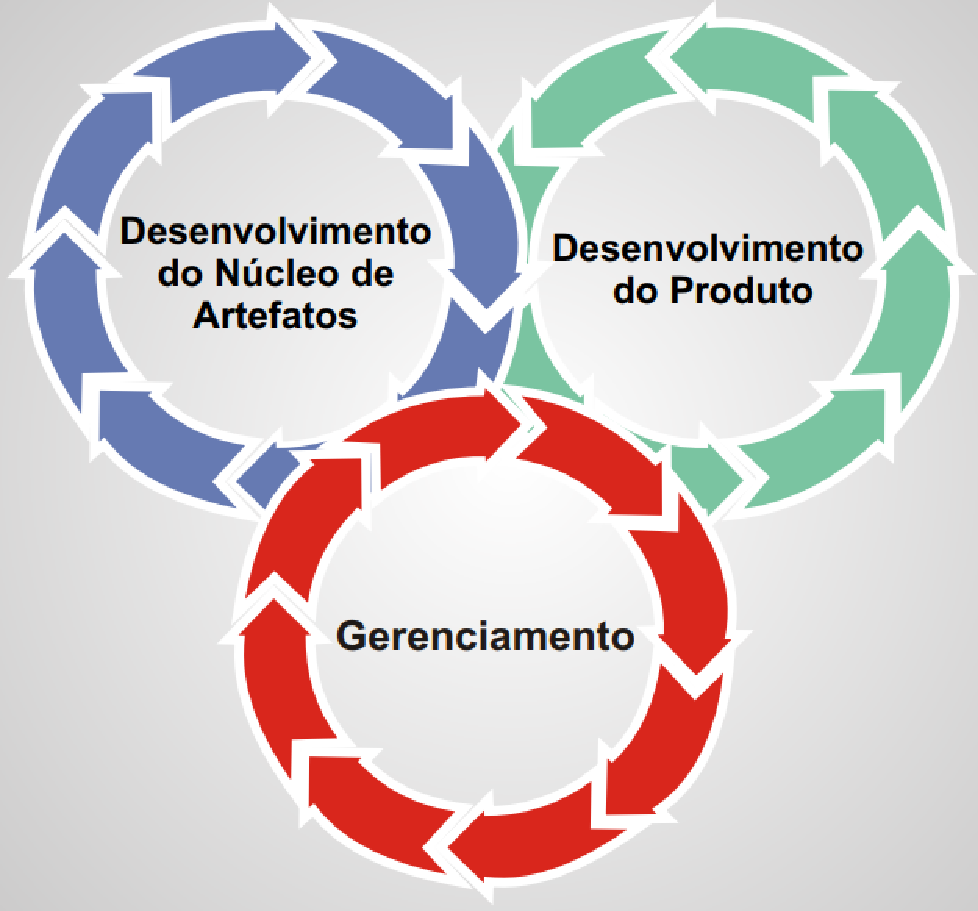
\includegraphics[scale=0.70]{sei.pdf}
	\caption{Adaptado de (SEI 2010) }
	\label{fig:sei}
\end{figure}

\begin{itemize}
	\item \textbf{Engenharia de Domínio} processo em que as similaridades e as variabilidades das LPSs são identificadas e realizadas. No qual, é composto de cinco subprocessos principais, sendo eles: Gerenciamento de Produto, Engenharia de Requisitos do Domínio, Projeto do Domínio, Realização do Domínio e Teste de Domínio;
	\item \textbf{Engenharia de Aplicação} processo em que as aplicações de uma LPS são construídas por meio da reutilização de artefatos de domínio, explorando as variabilidades de uma linha de produto. No qual, é composto pelas subprocessos: Engenharia de Requisitos da Aplicação, Projeto da Aplicação, Realização da Aplicação e Teste da Aplicação.
\end{itemize}

\cite{pohl2005software} desenvolveram um \textit{framework} para engenharia de LPS, cujo objetivo é incorporar os conceitos centrais da engenharia de linha de produto tradicional, proporcionando a reutilização de artefatos e a customização em massa por meio de variabilidades (\ref{fig:lps}).


\begin{figure}[htb]
	\centering
	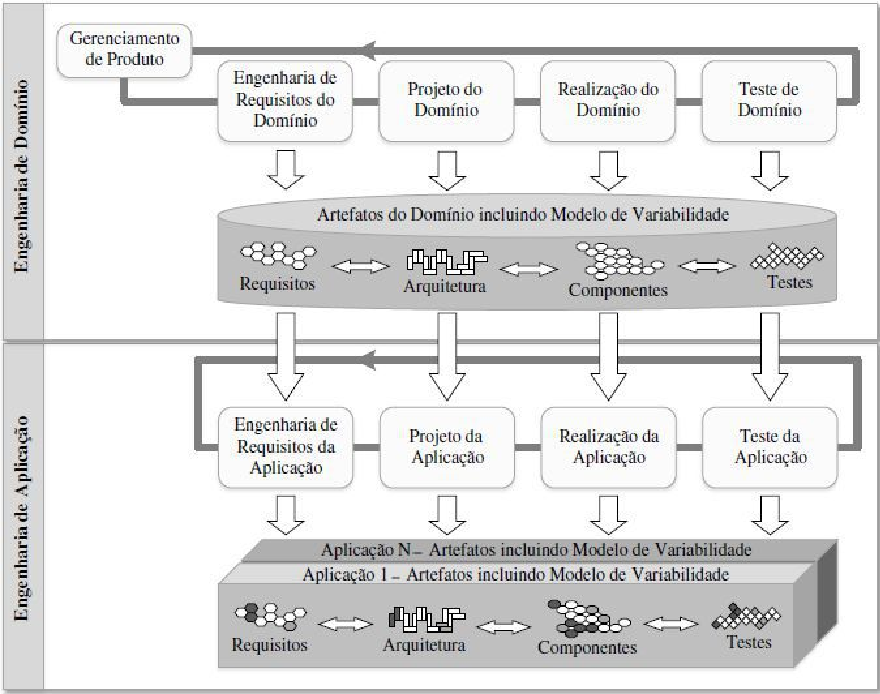
\includegraphics[scale=0.90]{lps.pdf}
	\caption{\textit{Framework} de Engenharia de LPS \cite{pohl2005software}. Traduzido por Geraldi (2015)}
	\label{fig:lps}
\end{figure}

A adoção de LPS traz benefícios em diversos aspectos do processo de desenvolvimento de software, tais como \cite{linden2007product, pohl2005software}:

\begin{itemize}
	\item redução dos custos de desenvolvimento, devido ao reúso de artefatos de um núcleo;
	\item melhoria da qualidade dos produtos, pois os artefatos produzidos são revisados e testados em vários produtos;
	\item redução do tempo de produção (\textit{time to market}) que é mais alto inicialmente, pois os artefatos comuns devem ser construídos antes. Mas, reduz ao produzir cada novo produto;
	\item redução do esforço de manutenção, pois quando um artefato do núcleo for modificado, as mudanças podem ser propagadas para todos os produtos que utilizam tal artefato;
	\item  contribuição para evolução, pois ao inserir um novo produto no núcleo da LPS, concede a oportunidade de evolução de todos os tipos de produtos derivados da LPS
	\item  contribuição para redução da complexidade, devido ao crescente número de solicitações de clientes, a complexidade dos produtos aumenta. Dessa forma, mais funcionalidades são adicionadas ao software. O fato de partes comuns serem 	reusadas por uma LPS ocorre a redução significativa da complexidade;
	\item melhoria na estimativa de custo, pois a organização pode se concentrar em promover produtos que são fáceis de ser gerados a partir da LPS e produtos que exijam extensões podem ser vendidos por preços mais altos; e 
	\item benefícios para os clientes, pois adquirem produtos adaptados às suas necessidades e expectativas por preços acessíveis devido a abordagem de LPS contribuir na redução de custos de desenvolvimento.
\end{itemize}

O núcleo de artefatos é composto de um conjunto de características comuns (similaridades) e características variáveis (variabilidades) \cite{linden2007product}. Esse núcleo forma a base da LPS e inclui a arquitetura de LPS, componentes reusáveis, modelos de domínios, requisitos da LPS, planos de testes e modelos de características e de variabilidades.

De acordo com \cite{apel2016feature}, "uma característica  é um comportamento visível ao usuário final de um sistema de software". Uma característica pode ser obrigatória, opcional ou alternativa. O modelo de características representa as variabilidades de uma LPS. Variabilidades são descritas por: Ponto de variação, o que permite a resolução de variabilidades em artefatos genéricos de uma LPS; Variante, que representa os possíveis elementos que podem ser escolhidos para resolver um ponto de variação e; Restrições entre variantes que estabelecem os relacionamentos entre uma ou mais variantes com o objetivo de resolver seus respectivos pontos de variação ou variabilidade em um dado tempo de resolução \cite{linden2007product,pohl2005software,apel2016feature}.

Analisando o contexto apresentado, podemos considerar que a variabilidade é algo muito importante para não ser levado em consideração quando falamos em qualidade de software. \textcolor{red}{Existem várias abordagens para o gerenciamento de variabilidade***citar quais são***}, uma delas é a \textit{Stereotype-based Management of Variability} (\textit{SMarty}), que realiza o gerenciamento de variabilidades de uma LPS de forma clara e explícita em modelos UML \cite{junior2010systematic}. \textit{SMarty} é composta de um perfil UML, o \textit{SMartyProfile}, e do processo denominado \textit{SMartyProcess}. Ela guia o usuário por meio do \textit{SMartyProcess} na identificação e representação de variabilidades em modelos UML de uma LPS. O perfil \textit{SMartyProfile} é formado por um conjunto de estereótipos e meta-atributos para representar variabilidades em modelos UML de LPS.

Por meio da UML e seu mecanismo de perfil \textit{SMarty} permite a representação explícita de variabilidades. O \textit{SMartyProcess} é um processo sistemático que guia o usuário na identificação, delimitação, representação, rastreamento de variabilidades e análise de configurações de produtos de uma LPS \textcolor{red}{explicar melhor essa figura (\ref{fig:smartyprocess}). e a 2.4 também} Nele há um conjunto de diretrizes que permitem ao usuário a aplicação dos estereótipos do \textit{SMartyProfile} de forma clara e objetiva e é possível perceber todos os estereótipos suportados pelo perfil na região inferior da (\ref{fig:smartyprofile}). Mais informações relacionadas a \textit{SMarty} podem ser encontradas no anexo \ref{Abordagem_SMarty} - Abordagem \textit{SMarty}, assim como um exemplo de modelagem utilizando a abordagem.

\begin{figure}[htb]
	\centering
	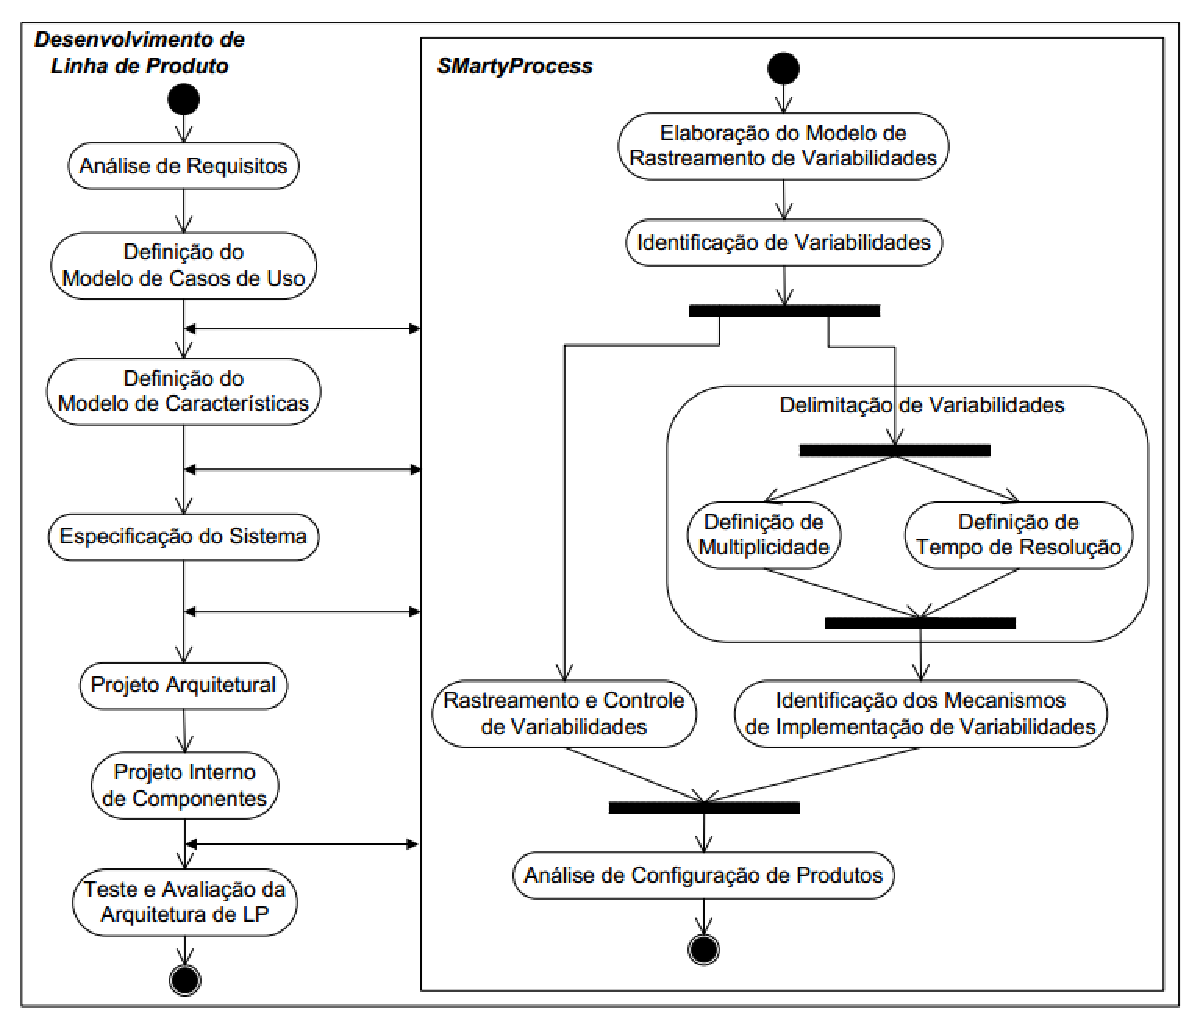
\includegraphics[scale=0.60]{smartyprocess.pdf}
	\caption{ O Processo de Gerenciamento de Variabilidades SMartyProcess e sua Interação entre as Atividades com o Processo de Desenvolvimento de LPS, traduzido de (OliveiraJr et al., 2010b)}
	\label{fig:smartyprocess}
\end{figure}


\begin{landscape}
	
	\begin{figure}[htb]
		\centering
		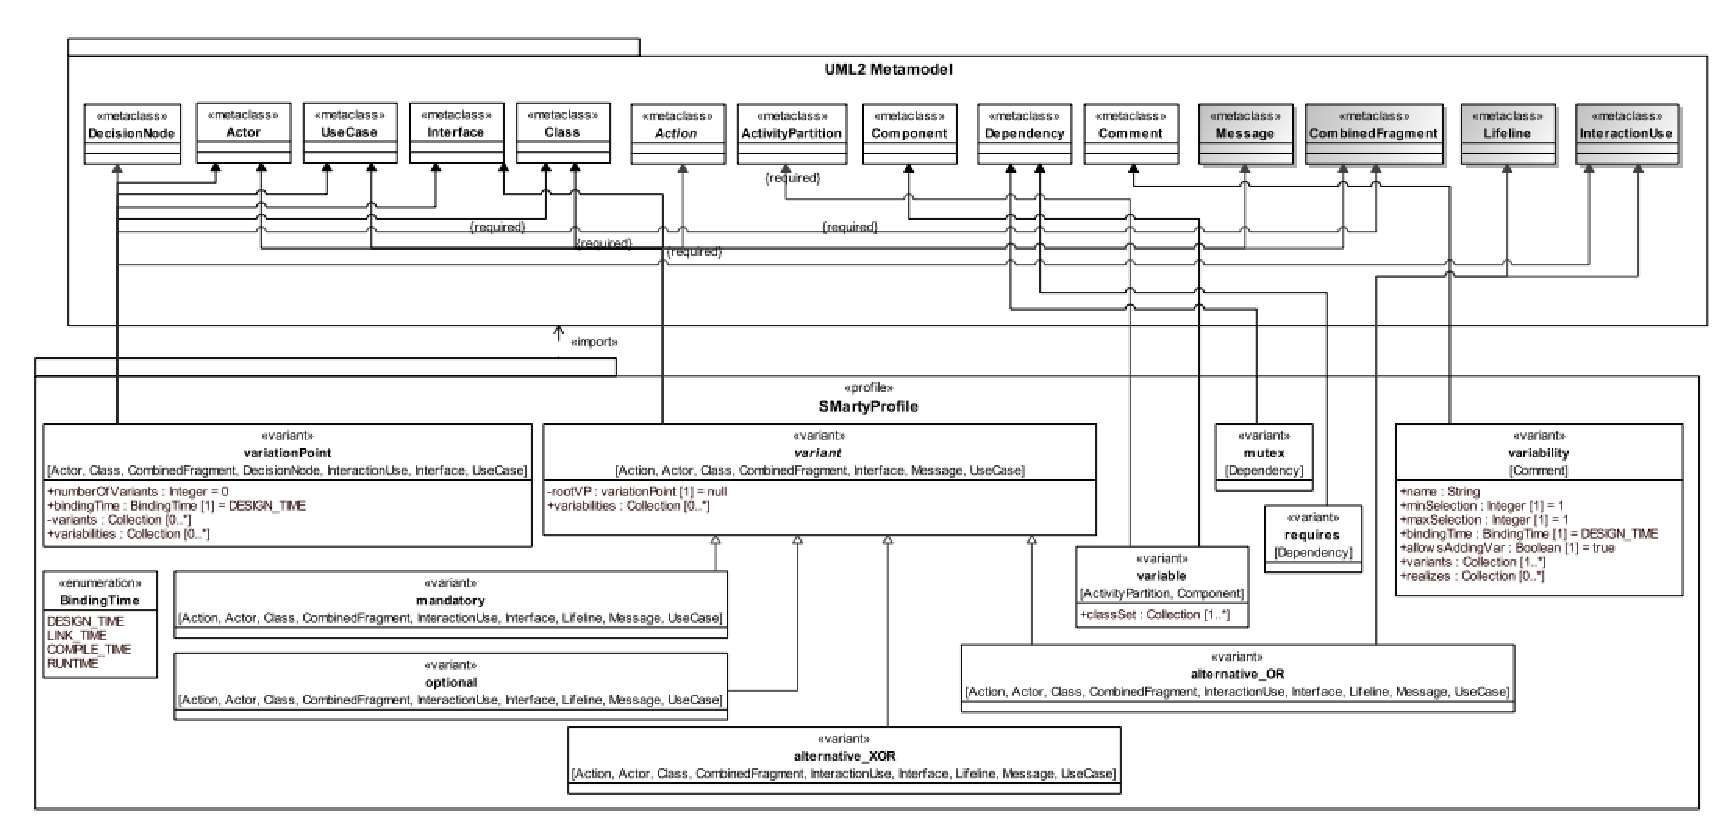
\includegraphics[scale=0.80]{smartyprofile.pdf}
		\caption{ Estereótipos e Meta-Atributos do Perfil SMartyProfile 5.1 com Suporte a Modelos de Casos de Uso, Classes, Componentes, Atividades e Sequência (Fiori et al., 2012; Marcolino, 2014; OliveiraJr et al., 2010a, 2013a). }
		\label{fig:smartyprofile}
	\end{figure}
	
	
\end{landscape}

\section{Teste de Linha de Produto de Software (LPS)}

contextualizar aqui os conceitos de teste

citar os principais itens da revisão sistemática que aborda testes em LPS

tentar contextualizar o teste de linha de produto de software com um exemplo em figura

\section{Teste baseado em Modelos para LPS}

LPS é um interesse da indústria pelo o potencial de reuso de artefatos além de aumentar a produtividade. Para alcançar as melhorias pretendidas, a qualidade dos artefatos reutilizáveis deve ser verificado. Portanto, a garantia de qualidade em geral. Testes em particular, ainda é a técnica de garantia de qualidade mais comum na indústria, são cruciais para os esforços de LPS \cite{delamaro2017introduccao}.

Sendo assim, para uma busca completa do desenvolvimento de teste em LPS primeiro temos que entender mais sobre o modelo de processo de teste. Atualmente existem vários modelos, porém, aqui iremos demonstrar um exemplo utilizando o modelo em V \ref{fig:testeV}.

\begin{figure}[htb]
	\centering
	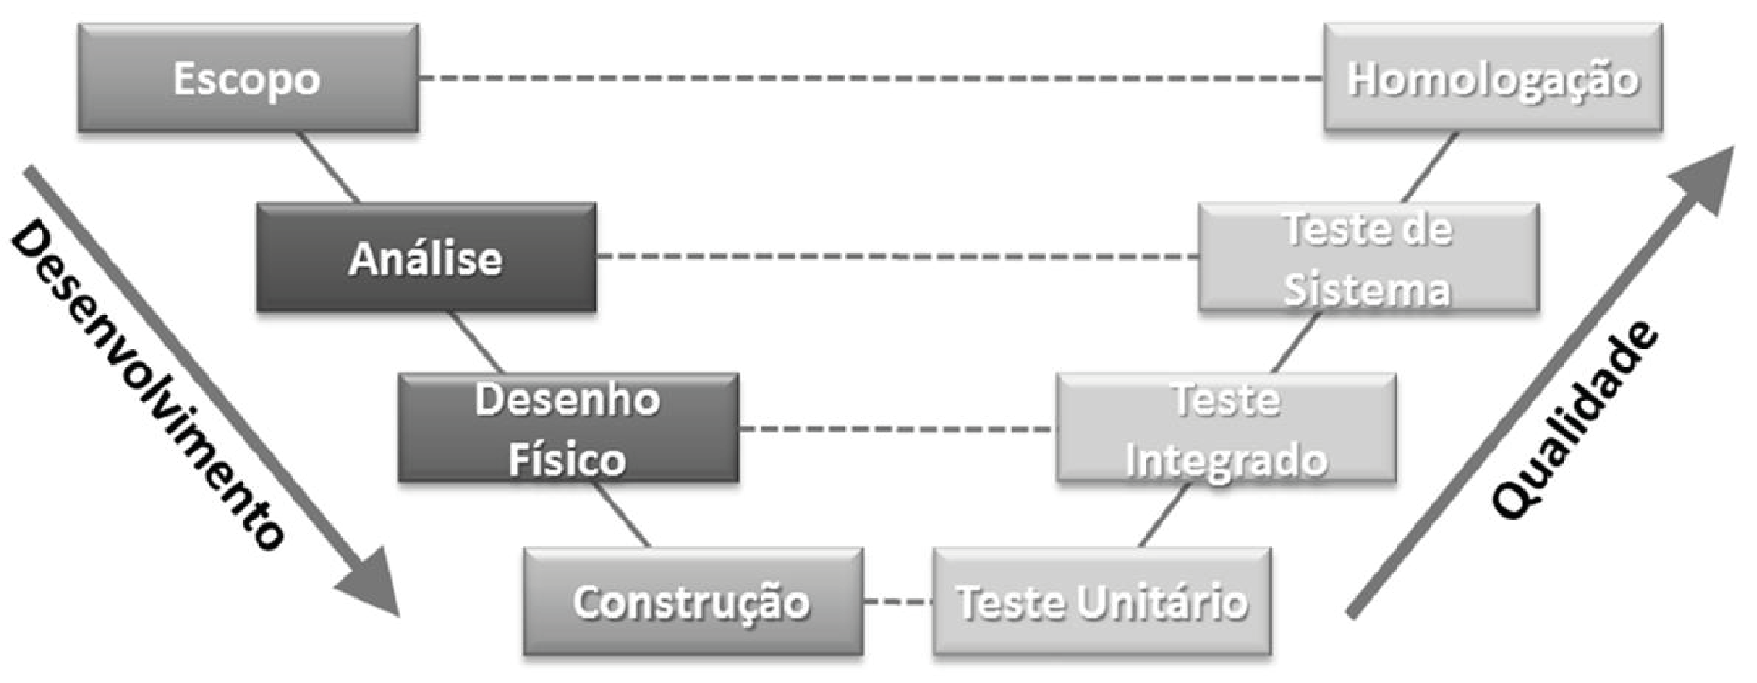
\includegraphics[scale=0.75]{teste.pdf}
	\caption{ Esquema simplificado que representa o modelo V }
	\label{fig:testeV}
\end{figure}

O modelo V é um modelo conceitual de Engenharia de sistemas/desenvolvimento de produto visto como melhoria ao problema de reatividade do modelo em cascata. Ele permite que, durante a integração de um sistema em seus diversos níveis, os testes sejam feitos contra os próprios requisitos do componente/interface que está sendo testado(a), em contraste com modelos anteriores onde o componente era testado contra a especificação do componente/interface.

Para este trabalho, a intenção é a antecipação dos testes como no modelo V \ref{fig:testeV} utilizando o modelo de teste consideramos duas etapas, a verificação e a validação. Aqui iremos tratar a validação, e por se tratar de teste de funcionalidade em engenharia de domínio, iremos utilizar a técnica de caixa preta,  onde em um processo de teste \ref{fig:testelps} na preparação do teste sabe-se apenas os parâmetros de entrada não temos acesso a parte interna do processo de execução, apenas o resultado esperado em sua saída para registro posterior do teste.


\begin{figure}[htb]
	\centering
	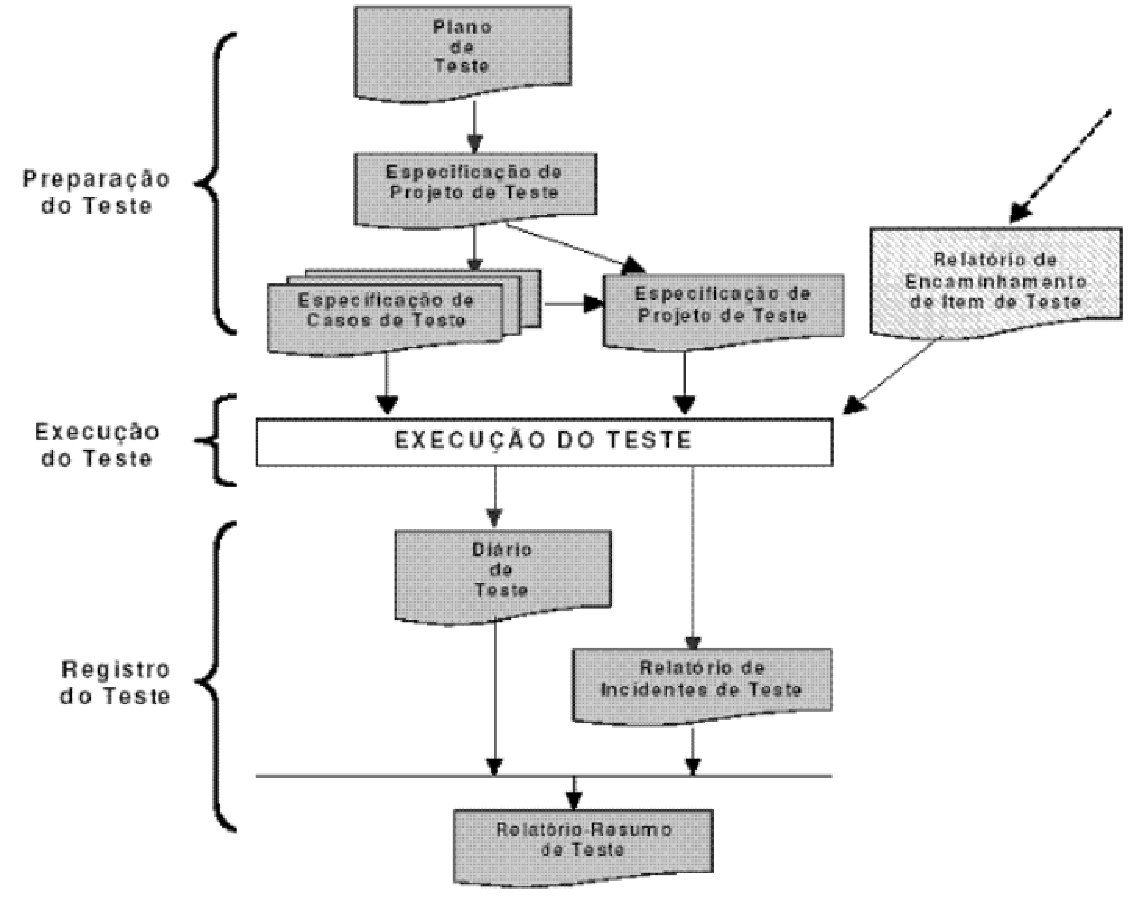
\includegraphics[scale=0.55]{testelps.pdf}
	\caption{ Modelo de proposta de implantação do processo de teste de software segundo \cite{crespo2004metodologia}}
	\label{fig:testelps}
\end{figure}

Sabendo-se que será utilizando teste caixa-preta, o nível de teste trabalhado poderá ser o de sistema, embora iremos trabalhar com diagramas mais detalhados como o de sequência. Pensando neste sentido de trabalho de teste a nível de engenharia de Domínio, procuramos buscar alternativas de teste que não necessitassem de atuação a nível de código ou caixa-branca.

\citealp{do2014strategies} cita em um trabalho de revisão de literatura relacionando teste em LPS, buscam analisar as estratégias de testes que são abordadas e quais seus potenciais em uma maior taxa de detecção de erros. Nesse casso eles apontam que testes devem ser considerados tanto na engenharia de domínio como na de aplicação. Dentro do interesse de teste dois itens devem ser levados em consideração, o conjunto de requisitos do produto e a qualidade do modelo de variabilidade em teste, isso demonstra que teste a nível de modelagem é uma item a ser pesquisado.

\citealp{do2014strategies} apresentam também um grande número de técnicas para lidar com o aspecto de seleção de produto para teste e o teste real dos produtos. No entanto, faltam relatos reais de experiências industriais que limitam algumas conclusões. O estudo ainda apresenta uma série de estratégias que podem apoiar a seleção e a execução dos testes reais em produtos.

O Teste Baseado em Modelo (TBM) é uma forma de teste de software em que os casos de teste são derivados de um modelo que descreve aspectos (geralmente funcionais) do sistema sendo testado. Tais casos são conhecidos como a suíte abstrata de testes, e seu nível de abstração está intimamente relacionado ao nível de abstração do modelo, segundo \citealp{do2014strategies}. As vantagens da abordagem é que a geração de testes começa mais cedo no ciclo do desenvolvimento e pode-se criar casos de teste automaticamente a partir do modelo, isso vai de encontro com nosso interesse, que é a antecipação da etapa de teste. 

Os casos de teste podem ser representados por meio de árvores de decisão, \textit{statecharts}, ontologias de domínio ou diagramas de casos de uso e/ou estados da UML (\textit{Unified Modeling Language})\cite{isa2017model}.

Baseado neste cenário, um dos maiores desafios em teste de LPS se dá em relação as particularidades de cada modelo, para isso TBM busca na criação de modelos dentro da engenharia de domínio, realizar a geração de casos de teste que possam ser reutilizados na engenharia de aplicação, foco da nossa pesquisa. Alguns trabalhos realizados focam na construção da geração antecipada dos teste na modelagem de domínio da LPS, onde, o foco das pesquisas ficam em relação a como conseguir gerar reutilização com uma maior cobertura dos possíveis problemas.

Uma particularidade de TBM é que ele se faz de uso de Máquinas de Estado Finito (MEF) \ref{fig:tbmmef}, um modelo formal que representa as possíveis configurações do sistema.

\begin{figure}[htb]
	\centering
	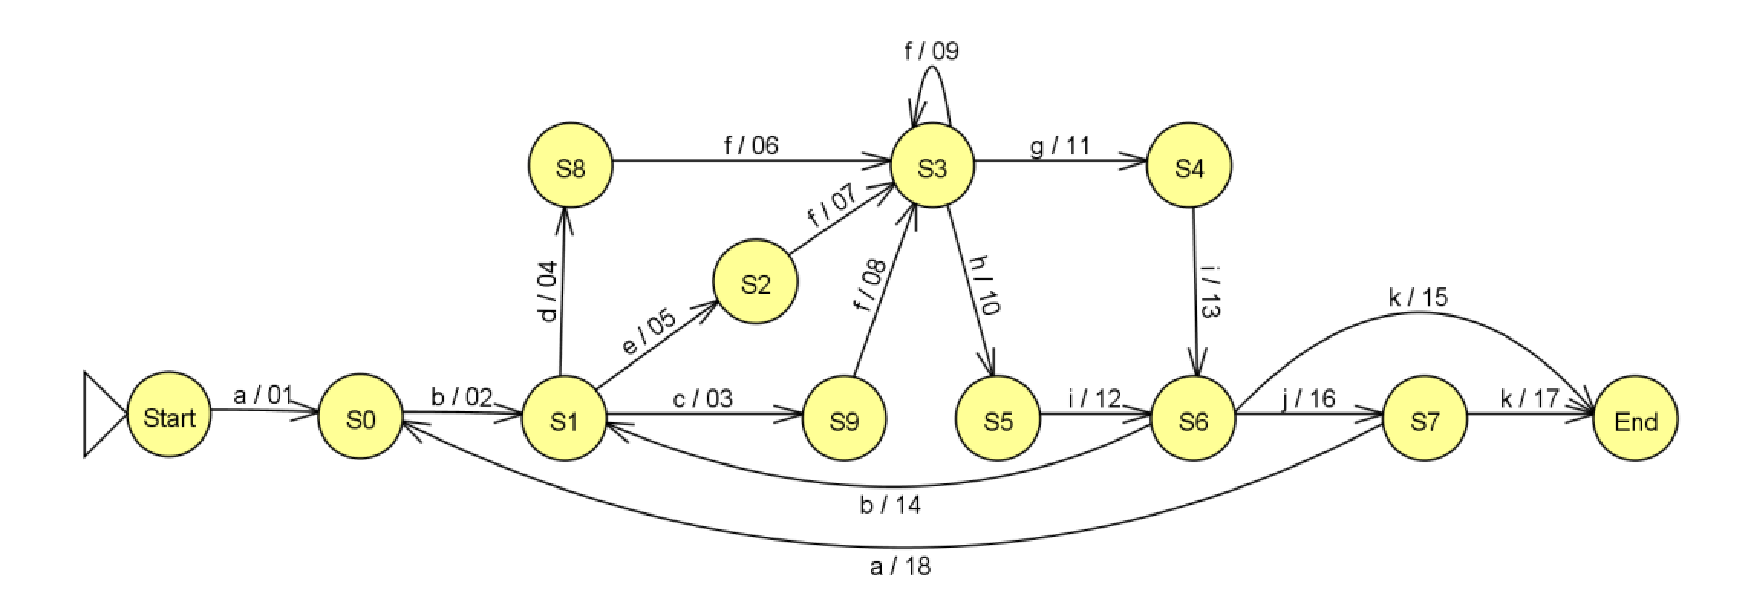
\includegraphics[scale=0.50]{fsm.pdf}
	\caption{ Exemplo de uma MEF utilizado por \citealp{costa2016split}}
	\label{fig:tbmmef}
\end{figure}

Sabendo que TBM possui características na utilização em LPS e que proporciona uma certa relação com variabilidade, preenchendo os principais requisitos para nossa pesquisa, foi conduzido um MSL Seção \ref{sec:MSL}, com a finalidade de evidenciar como que TBM esta sendo utilizado em LPS. Onde, ao longo de toda o MSL foram encontrados vários estudos que indicam a utilizam de TBM para LPS com tratativa da variabilidade.

Os estudos \textcolor{red}{quais estudos reportam do MSL} reportam que, em grande maioria, a partir de um modelo é realizado a conversão para um artefato, normalmente máquina de estado finito estendido, assim, ele pode ser verificado os pontos de variação e variabilidade. Após, gerenciado essa variabilidade com ou sem a utilização de uma ferramenta de apoio. E por fim, a criação do caso de teste, fazendo o uso ou não de rastreabilidade.

Para facilitar a leitura, os estudos utilizados para a extração de dados estão contidos na \ref{table:listaextraquali} que é um conjunto de estudos restante de todo o processo de mapeamento, e que reportam o TBM em LPS, assim foi criado um guia visual na \ref{fig:guiaestudo} onde apresenta um mapa com o que os trabalhos do MSL reportaram, contido na Anexo \ref{sec:roadmap} \textcolor{red}{*** reescrever ***}Porém, caso o leitor queira mais detalhes sobre o guia ou os trabalhos, ele pode consultar o MSL no Anexo \ref{sec:MSL}

A \ref{fig:guiaestudo} Apresenta um compilado de todos os trabalhos resultantes da MS organizados por tópicos chaves, considerando o interesse do leitor, um exemplo, caso o leitor queira saber quais trabalhos que utilizam de gerenciamento de variabilidade ele terá um item no gráfico apontando para este item.


\begin{landscape}
	\scalefont{0.7}
	\begin{longtable}[c]{|c|l|l|c|c|c|}
		\caption{Trabalhos selecionados para leitura e extração de dados}
		\label{table:listaextraquali}\\
		\hline
		\textbf{ID} & \multicolumn{1}{c|}{\textbf{Título}} & \multicolumn{1}{c|}{\textbf{Autor(res)}} & \textbf{\begin{tabular}[c]{@{}c@{}}Ano de \\ Publicação\end{tabular}} & \textbf{Fonte} & \textbf{Tipo} \\ \hline
		\endfirsthead
		%
		\hline
		\textbf{ID} & \multicolumn{1}{c|}{\textbf{Título}} & \multicolumn{1}{c|}{\textbf{Autor(res)}} & \textbf{\begin{tabular}[c]{@{}c@{}}Ano de \\ Publicação\end{tabular}} & \textbf{Fonte} & \textbf{Tipo} \\ \hline
		
		\endhead
		%
		T1 & \begin{tabular}[c]{@{}l@{}}Delta-Oriented Model-Based \\ SPL Regression Testing\end{tabular} & \begin{tabular}[c]{@{}l@{}}Sascha Lity, Malte Lochau, \\ Ina Schaefer, Ursula Goltz\end{tabular} & 2012 & ACM & Evento \\ \hline
		T2 & \begin{tabular}[c]{@{}l@{}}Industrial Evaluation of Pairwise \\ SPL Testing with MoSo-PoLiTe\end{tabular} & \begin{tabular}[c]{@{}l@{}}Michaela Steffens, Sebastian Oster, \\ Malte Lochau, Thomas Fogdal\end{tabular} & 2012 & ACM & Evento \\ \hline
		T3 & \begin{tabular}[c]{@{}l@{}}Model-Based Coverage-Driven Test Suíte \\ Generation for Software Product Lines\end{tabular} & \begin{tabular}[c]{@{}l@{}}Harald Cichos, Sebastian Oster, \\ Malte Lochau, Andy Schurr\end{tabular} & 2011 & ACM & Periódico \\ \hline
		T4 & \begin{tabular}[c]{@{}l@{}}MoSo-PoLiTe - Tool Support for \\ Pairwise and Model-Based Software \\ Product Line Testing\end{tabular} & \begin{tabular}[c]{@{}l@{}}Sebastian Oster, Ivan Zorcic, \\ Florian Markert, Malte Lochau\end{tabular} & 2011 & ACM & Evento \\ \hline
		T5 & MPLM - MaTeLo Product Line Manager & Hamza Samih, Ralf Bogusch & 2014 & ACM & Evento \\ \hline
		T6 & \begin{tabular}[c]{@{}l@{}}On the use of test cases in model-based \\ software product line development\end{tabular} & \begin{tabular}[c]{@{}l@{}}Alexander Knapp, Markus Roggenbach, \\ Bernd-Holger Schlingloff\end{tabular} & 2014 & ACM & Evento \\ \hline
		T7 & \begin{tabular}[c]{@{}l@{}}Pairwise Feature-Interaction Testing \\ for SPLs: Potentials and Limitations\end{tabular} & \begin{tabular}[c]{@{}l@{}}Sebastian Oster, Malte Lochau, \\ Marius Zink, Mark Grechanik\end{tabular} & 2011 & ACM & Evento \\ \hline
		T8 & \begin{tabular}[c]{@{}l@{}}Deriving Usage Model Variants for \\ Model- based Testing: An Industrial Case Study\end{tabular} & \begin{tabular}[c]{@{}l@{}}Hamza Samih,  Hélène Le Guen, \\ Ralf Bogusch, Mathieu Acher, Benoit Baudry\end{tabular} & 2014 & IEEE & Evento \\ \hline
		T9 & \begin{tabular}[c]{@{}l@{}}Model-based Software Product Line \\ Testing by Coupling Feature Models \\ with Hierarchical Markov Chain Usage Models\end{tabular} & Ceren Sahin Gebizli, Hasan Sozer & 2016 & IEEE & Evento \\ \hline
		T10 & \begin{tabular}[c]{@{}l@{}}Model-Based Test Design of Product Lines: \\ Raising Test Design to the Product Line Level\end{tabular} & \begin{tabular}[c]{@{}l@{}}Hartmut Lackner, Martin Thomas, \\ Florian Wartenberg, Stephan Weißleder\end{tabular} & 2014 & IEEE & Periódico \\ \hline
		T11 & Requirements-Based Delta-Oriented SPL Testing & \begin{tabular}[c]{@{}l@{}}Michael Dukaczewski, Ina Schaefer, \\ Remo Lachmann, Malte Lochau\end{tabular} & 2013 & IEEE & Evento \\ \hline
		T12 & \begin{tabular}[c]{@{}l@{}}Using Feature Model to Support Model- Based \\ Testing of Product Lines: An Industrial Case Study\end{tabular} & \begin{tabular}[c]{@{}l@{}}Shuai Wang,  Shaukat Ali,\\  Tao Yue, Marius Liaaen\end{tabular} & 2013 & IEEE & Periódico \\ \hline
		T13 & \begin{tabular}[c]{@{}l@{}}An automated Model-based Testing \\ Approach in Software Product Lines \\ Using a Variability Language\end{tabular} & \begin{tabular}[c]{@{}l@{}}Boni García,  Rodrigo García-Carmona, \\ Álvaro Navas, Hugo A. Parada-Gélvez,\\  Félix Cuadrado, Juan C. Dueñas\end{tabular} & 2010 & \begin{tabular}[c]{@{}c@{}}Politécnica \\ Arquivo \\ digital UPM\end{tabular} & Evento \\ \hline
		T14 & \begin{tabular}[c]{@{}l@{}}Automated Product Line Methodologies \\ to Support Model-Based Testing\end{tabular} & Shuai Wang,  Shaukat Ali, Arnaud Gotlieb & 2013 & \begin{tabular}[c]{@{}c@{}}CEUR \\ Event Proceedings\end{tabular} & Evento \\ \hline
		T15 & \begin{tabular}[c]{@{}l@{}}Behavioural Model Based \\ Testing of Software Product Lines\end{tabular} & Xavier Devroey & 2014 & ACM & Evento \\ \hline
		T16 & \begin{tabular}[c]{@{}l@{}}Feature Model-based \\ Software Product Line Testing\end{tabular} & SEBASTIAN OSTER & 2012 & TUprints & Periódico \\ \hline
		T17 & \begin{tabular}[c]{@{}l@{}}Model-based pairwise testing for feature interaction \\ coverage in software product line engineering\end{tabular} & \begin{tabular}[c]{@{}l@{}}Malte Lochau, Sebastian Oster, \\ Ursula Goltz, Andy Schurr\end{tabular} & 2011 & Springer & Periódico \\ \hline
		T18 & Model-based Test Generation for Software Product Line & Xinying Cai, Hongwei Zeng & 2013 & IEEE & Evento \\ \hline
		T19 & Model-Based Testing for Software Product Lines & Erika Mir Olimpiew & 2008 & Springer & Evento \\ \hline
		T20 & PLETS - A Product line of model-based testing tools & Elder de Macedo Rodrigues & 2013 & PUC-RS & Evento \\ \hline
		T21 & \begin{tabular}[c]{@{}l@{}}Top-Down and Bottom-Up Approach for \\ Model-Based Testing of Product Lines\end{tabular} & Stephan Weißleder, Hartmut Lackner & 2013 & EPTCS & Evento \\ \hline
		T22 & \begin{tabular}[c]{@{}l@{}}A Product Line Modeling and Configuration  Methodology \\ to Support Model-Based  Testing: An Industrial Case Study\end{tabular} & \begin{tabular}[c]{@{}l@{}}Shaukat Ali, Tao Yue, Lionel Briand, \\ Suneth Walawege\end{tabular} & 2012 & Springer & Periódico \\ \hline
		T23 & \begin{tabular}[c]{@{}l@{}}Coverage Criteria for Behavioural \\ Testing of Software Product Lines\end{tabular} & \begin{tabular}[c]{@{}l@{}}Xavier Devroey, Gilles Perrouin, \\ Axel Legay, Maxime Cordy, \\ Pierre-Yves Schobbens, Patrick Heymans\end{tabular} & 2014 & Springer & Evento \\ \hline
		T24 & \begin{tabular}[c]{@{}l@{}}A Model Based Testing Approach for Model-Driven \\ Development and Software Product Lines\end{tabular} & \begin{tabular}[c]{@{}l@{}}Beatriz Pérez Lamancha,  Macario Polo Usaola, \\ Mario Piattini Velthius\end{tabular} & 2010 & Springer & Evento \\ \hline
		T25 & \begin{tabular}[c]{@{}l@{}}A Vision for Behavioural Model-Driven \\ Validation of Software Product Lines\end{tabular} & \begin{tabular}[c]{@{}l@{}}Xavier Devroey, Maxime Cordy,  \\ Gilles Perrouin, Eun-Young Kang, \\ Pierre-Yves Schobbens, Patrick Heymans, \\ Axel Legay,  Benoit Baudry\end{tabular} & 2012 & Springer & Evento \\ \hline
		T26 & \begin{tabular}[c]{@{}l@{}}Abstract Test Case Generation for Behavioural \\ Testing of Software Product Lines\end{tabular} & \begin{tabular}[c]{@{}l@{}}Xavier Devroey, Gilles Perrouin, \\ Pierre-Yves Schobbens\end{tabular} & 2014 & ACM & Evento \\ \hline
		T27 & \begin{tabular}[c]{@{}l@{}}Applying Incremental Model Slicing to \\ Product-Line Regression Testing\end{tabular} & \begin{tabular}[c]{@{}l@{}}Sascha Lity, Thomas Morbach,  \\ Thomas Th¨ um, Ina Schaefer\end{tabular} & 2016 & Springer & Periódico \\ \hline
		T28 & \begin{tabular}[c]{@{}l@{}}Automated Testing of Software-as- a-Service \\ Configurations using a Variability Language\end{tabular} & Sachin Patel, Vipul Shah & 2015 & ACM & Evento \\ \hline
		T29 & Delta-Oriented FSM-Based Testing & \begin{tabular}[c]{@{}l@{}}Mahsa Varshosaz,  Harsh Beohar, \\ Mohammad Reza Mousavi\end{tabular} & 2015 & Springer & Evento \\ \hline
		T30 & \begin{tabular}[c]{@{}l@{}}Incremental Model-Based Testing of \\ Delta-oriented Software Product Lines\end{tabular} & \begin{tabular}[c]{@{}l@{}}Malte Lochau, Ina Schaefer, \\ Jochen Kamischke, Sascha Lity\end{tabular} & 2012 & Springer & Periódico \\ \hline
		T31 & Model Based Testing in Software Product Lines & \begin{tabular}[c]{@{}l@{}}Pedro Reales, Macario Polo, \\ Danilo Caivano\end{tabular} & 2011 & Springer & Evento \\ \hline
		T32 & Model-Based Testing & \begin{tabular}[c]{@{}l@{}}Malte Lochau, Sven Peldszus, \\ Matthias Kowal,  Ina Schaefer\end{tabular} & 2014 & Springer & Evento \\ \hline
		T33 & \begin{tabular}[c]{@{}l@{}}Parameterized Preorder Relations for \\ Model-Based Testing of Software Product Lines\end{tabular} & Malte Lochau, Jochen Kamischke & 2012 & Springer & Evento \\ \hline
		T34 & Poster: VIBeS, Transition System Mutation Made Easy & \begin{tabular}[c]{@{}l@{}}Xavier Devroey, Gilles Perrouin, \\ Pierre-Yves Schobbens, Patrick Heymans\end{tabular} & 2015 & IEEE & Evento \\ \hline
		T35 & Spinal Test Suites for Software Product Lines & Harsh Beohar, Mohammad Reza Mousavi & 2014 & EPTCS & Evento \\ \hline
		T36 & \begin{tabular}[c]{@{}l@{}}Automated model-based testing\\ using the  UML testing profile and QVT\end{tabular} & \begin{tabular}[c]{@{}l@{}}Beatriz Pérez Lamancha, Pedro Reales Mateo, \\ IgnacioRodríguez de Guzmán, Macario Polo Usaola, \\ Mario Piattini Velthius\end{tabular} & 2009 & ACM & Evento \\ \hline
		T37 & \begin{tabular}[c]{@{}l@{}}Relating Variability Modeling and \\ Model- Based Testing for Software Product Lines Testing\end{tabular} & Hamza Samih & 2012 & ICTSS & Evento \\ \hline
		T38 & \begin{tabular}[c]{@{}l@{}}An Evaluation of Model-Based \\ Testing in Embedded Applications\end{tabular} & Stephan Weißleder, Holger Schlingloff & 2014 & IEEE & Evento \\ \hline
		T39 & \begin{tabular}[c]{@{}l@{}}Assessing Software Product Line Testing Via Model-Based \\ Mutation An Application to Similarity Testing\end{tabular} & \begin{tabular}[c]{@{}l@{}}Christopher Henard, Mike Papadakis, \\ Gilles Perrouin, Jacques Klein, Yves Le Traon\end{tabular} & 2013 & IEEE & Evento \\ \hline
		T40 & \begin{tabular}[c]{@{}l@{}}Automated and Scalable T-wise Test Case Generation \\ Strategies for Software Product Lines\end{tabular} & \begin{tabular}[c]{@{}l@{}}Gilles Perrouin, Sagar Sen, Jacques Klein, \\ Benoit Baudry, Yves le Traon Lassy\end{tabular} & 2010 & IEEE & Evento \\ \hline
		T41 & \begin{tabular}[c]{@{}l@{}}Model-based Testing of System Requirements \\ using UML Use Case Models\end{tabular} & Bill Hasling, Helmut Goetz, Klaus Beetz & 2008 & IEEE & Evento \\ \hline
		T42 & \begin{tabular}[c]{@{}l@{}}Successive refinement of models for model-based \\ testing to increase system test effectiveness\end{tabular} & \begin{tabular}[c]{@{}l@{}}Ceren Sahin Gebizli, Hasan Sozer, \\ Ali Ozer Ercan\end{tabular} & 2016 & IEEE & Evento \\ \hline
		T43 & A Software Product Line for Model-Based Testing Tools & \begin{tabular}[c]{@{}l@{}}Elder M. Rodrigues, Avelino F. Zorzo, \\ Itana M. Gimenez, Elisa Y. Nakagawa, \\ Flavio M. Oliveira, José C. Maldonado\end{tabular} & 2012 & PUC-RS & Outro \\ \hline
		T44 & \begin{tabular}[c]{@{}l@{}}Reusing State Machines for Automatic \\ Test Generation in Product Lines\end{tabular} & \begin{tabular}[c]{@{}l@{}}Stephan Weißleder, Dehla Sokenou, \\ Bernd-Holger Schlingloff\end{tabular} & 2008 & MoTip & Evento \\ \hline
	\end{longtable}
\end{landscape}

%\begin{landscape}
	
%	\begin{figure}[htb]
%		\centering
%		\caption{Atualizar imagem Guia de estágios do processo de TBM em LPS}
%		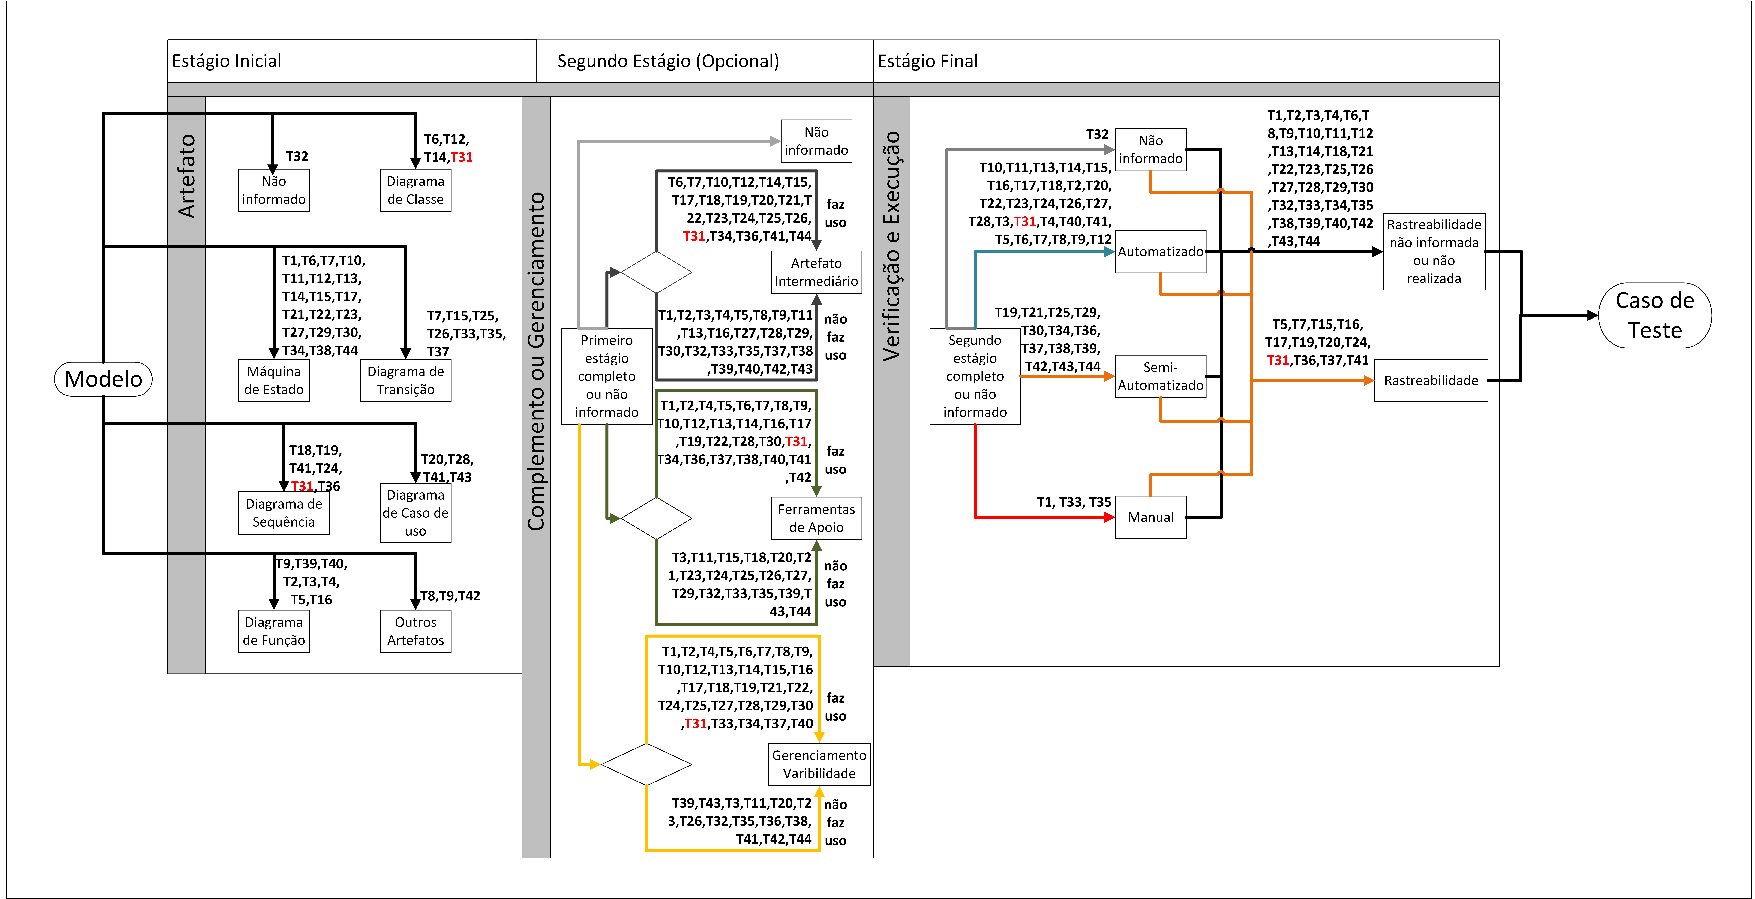
\includegraphics[scale=0.40]{guiaestudo.png}
%		\label{fig:guiaestudoquali}
%	\end{figure}
%	
%\end{landscape}

\section{A Abordagem SPLit-MbT}

\cite{costa2016split} apresenta uma abordagem denominada \textit{Software Product Line Testing Method Based on System Models} (SPLiT-MBt) onde é possível gerar casos de teste funcional e \textit{scripts} para testar os produtos derivados de uma LPS, onde os casos de teste comuns entre os produtos derivados são gerados com base no reuso inerente a LPS.

\begin{figure}[htb]
	\centering
	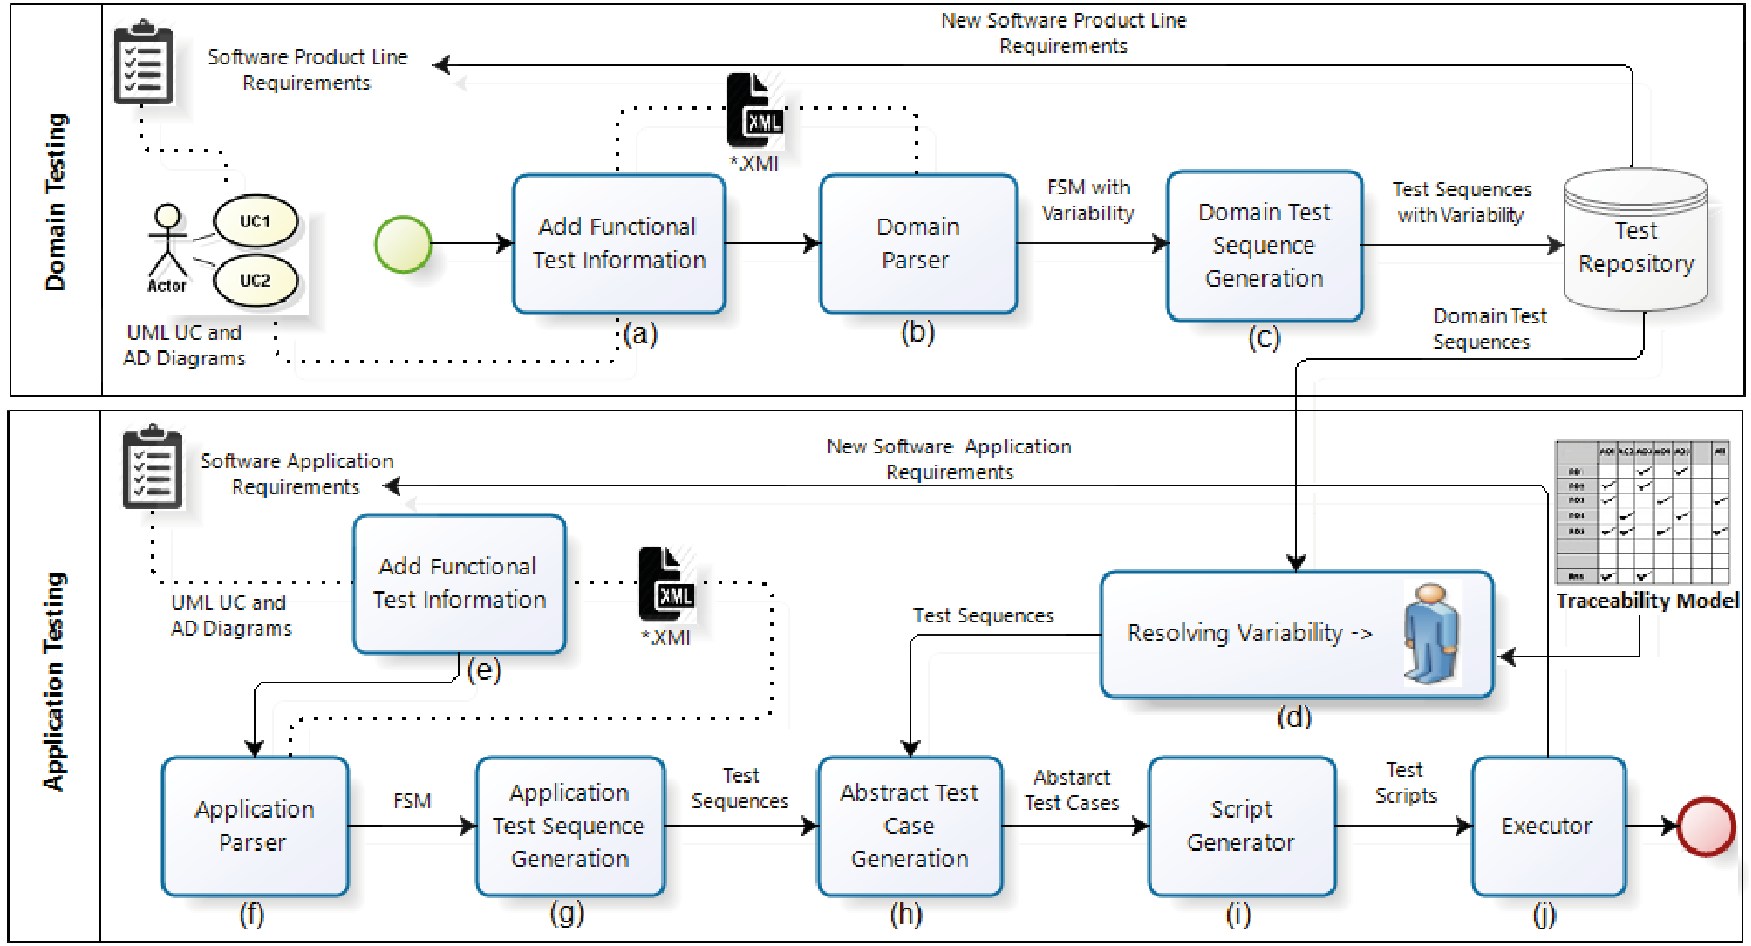
\includegraphics[scale=0.60]{splitmbt.pdf}
	\caption{Panorama da abordagem SPLiT-MBt por \citealp{costa2016split}}
	\label{fig:splitmbt}
\end{figure}

O objetivo principal da abordagem é prover o reuso de artefatos de teste baseado na adaptação do uso de teste baseado em modelo (TBM) para geração automática de casos de teste funcional e \textit{scripts} para modelos considerando a variabilidade.

Para fornecer o reuso ele é aplicado em duas etapas vide \ref{fig:splitmbt}, onde na primeira é realizada a anotação em modelo de sistema, as informações de variabilidade e teste, em seguida utilizadas para gerar sequências de teste usando diferentes métodos formais, como o HSI, UIO,DS ou TT. O modelo formal utilizado é Máquina de Estado Finito e que são estendidas para lidar com as informações sobre variabilidade, uma vez que os modelos de entrada esperado é que já esteja modelado com base na abordagem \textit{SMarty}.

Na engenharia de domínio um diagrama de atividade é convertido em uma Máquina de estado Finitos (MEF) onde é estendida para lidar com informações sobre variabilidade, em seguida se faz a utilização de um modelo formal de geração de sequência de teste denominado HSI. Então essas sequências de teste são armazenadas em um repositório para reutilização, porém, ainda sem a resolução da variabilidade.

Já na segunda etapa, na engenharia de aplicação, os casos de teste são reaproveitados e assim é gerado uma solução para a variabilidade, os modelos de teste e as sequências geradas são utilizadas para gerar os \textit{scripts} de teste que podem ser executados por diferentes ferramentas de teste funcional. Outro fator que deve ser levado em consideração é a rastreabilidade dos casos de teste, que proporciona uma verificação posterior de quais casos de teste foram reaproveitados e se sofreram atualizações. as diferenças entre este trabalho para com o SPLiT-MBt é que \textit{SMartyTesting} dará suporte ao diagrama de sequência que também é suportado por \textit{SMarty}, a escolha por este tipo de modelo é por proporcionar um maior teor de detalhes relacionado aos processos.

\section{Considerações Finais}
Nesta seção não foi abordado alguns temas como tipos, técnicas ou níveis de teste, pois entendemos que o leitor que venha buscar por este assunto já está familiarizado com os princípios básicos de teste de software.

